\documentclass[tikz,border=8pt]{standalone}
% Shared look for every TikZ diagram. Load with \input{../../tools/tikz-style.tex}
\usepackage[sfdefault]{roboto}
\usetikzlibrary{arrows.meta, positioning, shapes.geometric, calc, fit, backgrounds}
\definecolor{cblue}{HTML}{4C78A8}
\definecolor{corange}{HTML}{F58518}
\definecolor{cgreen}{HTML}{54A24B}
\definecolor{cred}{HTML}{E45756}
\definecolor{cpurple}{HTML}{B279A2}
\definecolor{cgrey}{HTML}{6B6B6B}
\tikzset{
  every picture/.style={font=\sffamily, line width=1.2pt},
  box/.style={draw=#1, fill=#1!12, rounded corners=4pt, align=center, inner sep=7pt, minimum height=1.1cm},
  box/.default=cgrey,
  arrow/.style={-{Stealth[length=3mm]}, draw=cgrey, line width=1.4pt},
  title/.style={font=\sffamily\bfseries\Large},
  note/.style={font=\sffamily\small, text=cgrey, align=center},
}
\AtBeginDocument{\hyphenpenalty=10000 \exhyphenpenalty=10000}

% The speed controller this Note builds, each piece tagged with its section: the planner's command passes the
% velocity smoother (rate limit, deadband), the feedforward computes the force the plan needs, the PI loop with
% anti-windup corrects the rest, the drive limits the force to +-4 N, and the robot's speed is fed back.
\begin{document}
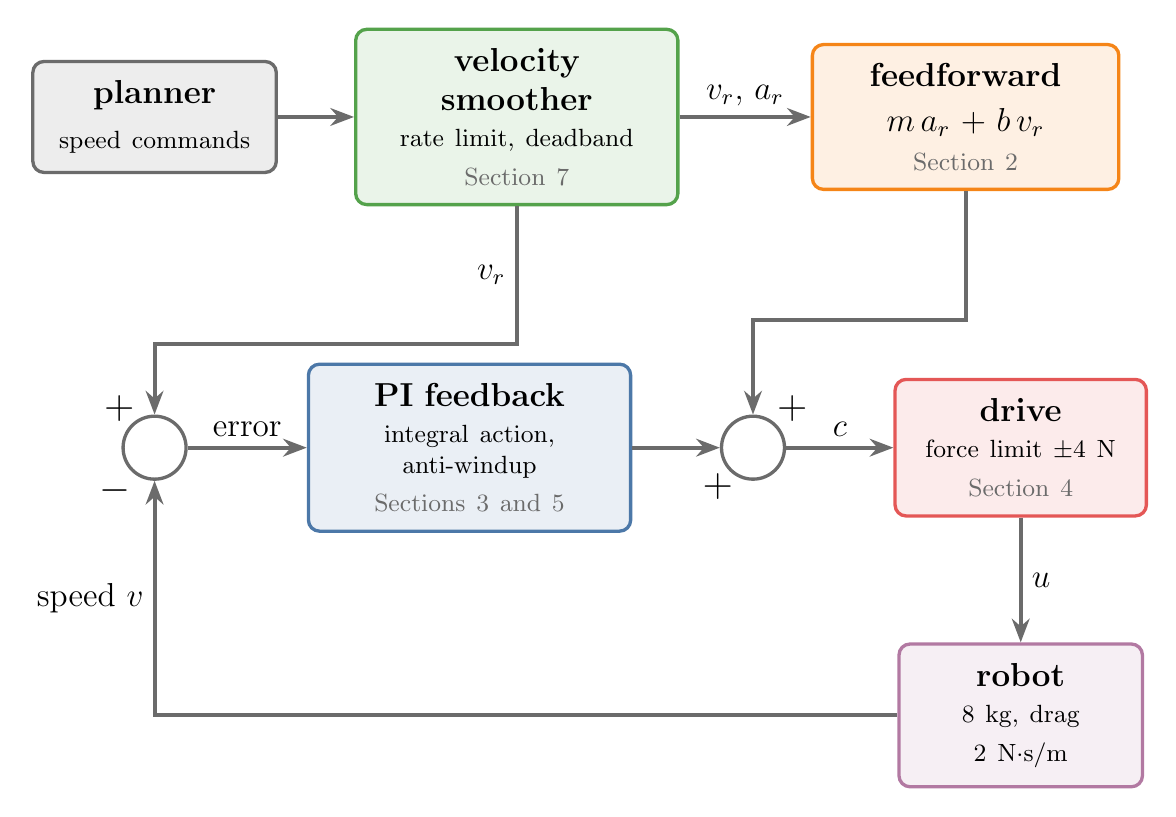
\begin{tikzpicture}[every node/.append style={font=\large}]
  \node[box=cgrey, text width=2.6cm] (plan) at (0,4.2) {\textbf{planner}\\[2pt] \small speed commands};
  \node[box=cgreen, text width=3.6cm] (smooth) at (4.6,4.2) {\textbf{velocity smoother}\\[2pt]
     \small rate limit, deadband\\ \textcolor{cgrey}{Section 7}};
  \node[box=corange, text width=3.4cm] (ff) at (10.3,4.2) {\textbf{feedforward}\\[2pt] $m\,a_r + b\,v_r$\\
     \small\textcolor{cgrey}{Section 2}};
  \node[circle, draw=cgrey, fill=white, minimum size=0.8cm, inner sep=0pt] (err) at (0,0) {};
  \node[box=cblue, text width=3.6cm] (pi) at (4.0,0) {\textbf{PI feedback}\\[2pt] \small integral action,
     anti-windup\\ \textcolor{cgrey}{Sections 3 and 5}};
  \node[circle, draw=cgrey, fill=white, minimum size=0.8cm, inner sep=0pt] (sum) at (7.6,0) {};
  \node[box=cred, text width=2.7cm] (drive) at (11.0,0) {\textbf{drive}\\[2pt] \small force limit $\pm$4 N\\
     \textcolor{cgrey}{Section 4}};
  \node[box=cpurple, text width=2.6cm] (robot) at (11.0,-3.4) {\textbf{robot}\\[2pt] \small 8 kg, drag\\ 2 N$\cdot$s/m};
  \draw[arrow] (plan) -- (smooth);
  \draw[arrow] (smooth) -- node[above] {$v_r$, $a_r$} (ff);
  \draw[arrow] (smooth.south) |- node[pos=0.25, left] {$v_r$} ($(err.north)+(0,0.9)$) -- (err.north);
  \node[font=\Large] at ($(err.north west)+(-0.15,0.2)$) {$+$};
  \draw[arrow] (err) -- node[above] {error} (pi);
  \draw[arrow] (pi) -- (sum);
  \draw[arrow] (ff.south) |- ($(sum.north)+(0,1.2)$) -- (sum.north);
  \draw[arrow] (sum) -- node[above] {$c$} (drive);
  \node[font=\Large] at ($(sum.north east)+(0.2,0.2)$) {$+$};
  \node[font=\Large] at ($(sum.south west)+(-0.15,-0.2)$) {$+$};
  \draw[arrow] (drive) -- node[right] {$u$} (robot);
  \draw[arrow] (robot.west) -| node[pos=0.75, left] {speed $v$} (err.south);
  \node[font=\Large] at ($(err.south west)+(-0.2,-0.25)$) {$-$};
\end{tikzpicture}
\end{document}
